\documentclass[11pt]{article}

\usepackage[utf8]{inputenc}
\usepackage[x11names]{xcolor}   % Accès à une table de 317 couleurs
\usepackage{graphicx} %Pour utiliser la colorbox et les images
\usepackage{textcomp}
\usepackage{amsmath}
\usepackage{amssymb}
\usepackage[ruled]{algorithm2e}

\title{\textbf{CPA \\ étude de l'algorithme de Erno Welzl pour le cercle minimum.}}
\author{RETAIL Tanguy}
\date{25/02/2016}
\begin{document}

\maketitle
\tableofcontents
\newpage

\section{Introduction}
Etant donné un ensemble de points dans le plan carétsien, nous cherchons le cercle minimum qui contienne tous ces points, ce cercle est unique. Ce problème fût proposé par mathématicien anglais James Joseph Sylvester en 1857. 
De nombreuses solutionsfurent proposées pour calculer le cercle minimum, dans un temps généralement O($n^2$), on peut citer Elzinga and Hearn en 1972, Shamos and Hoey en 1975, et finalement Preparata en 1977. Shamos découvrit en 1978 le premier algorithme en O(n logn).
Nimrod Megiddo en 1983 proposa un premier algo linéaire, assez fastidieux. Il faut attendre 1991 pour l'algorithme de Welzl qui calcule le cercle minimum d'une manière simple à partir d'un nuage de points dans un temps théorique quadratique, mais linéaire expérimentalement.

\subsection{Définition cercle minimum}
Le cercle minimum est défini pour un ensemble d'au moins deux points. En effet le cercle minimum pour un point, est ce point lui-même. Le cercle minimum est donc caractérisé par soit deux points sur le cercle, diamétralement opposés, soit par un cercle circonscrit (passant par au moins trois points, cocirculaires).

\subsubsection{Unicité du cercle minimum}
Soient deux cercle $C_1$ et $C_2$ deux cercles minimaux différents du même ensemble de points S. Alors leur intersection $I \subseteq C_1 \cap C_2$ contient S. Le cercle passant par les intersections $i_1$ et $i_2$ des deux cercles et de centre $(\dfrac{i_{1x} + i_{2x}}{2},\dfrac{i_{1y} + i_{2y}}{2})$ a un rayon nécessairement plus petit. C'est une contradiction, le cercle minimum est unique.
\subsubsection{Caractérisation du cercle minimum}
Selon Welzl [1] :
Soit P un ensemble de n points, P non vide et p est un point dans P. R est également un ensemble de points, qui sont en fait les points sur le cercle. Le lemme dit : \\
(i) Si il existe un cercle contenant P avec R sur ce cercle, alors D(P,R) est unique.\\
(ii) Si p n'appartient pas à D(P - {p},R), alors p est sur le cercle D(P,R) = D(P - {p}, R u {p}).\\
(iii) Si D(P,R) existe, il existe un ensemble S d'au plus {0, 3 - $\|$R$\|$} points dans P tel que D(P,R) = D(S,R). Ce qui implique que P est caractérisé par au plus 3 points dans P qui sont sur le cercle D(P).
\subsection{Algorithme naïf}
Cet algorithme, supposé exact, nous servira de référence afin de valider nos résultats avec l'agorithme de Welzl lors des expérimentations.\\
Le principe est le suivant :\\
Nous testons toutes les paires de point dans l'ensemble, espérant trouver un cercle qui contienne tous les points. Si ce cercle existe, alors il est minimal. Tester chaque paire est quadratique, tester l'appartenance de l'ensemble est linéaire. Le cercle est alors trouvé en $\mathcal{O}(n^3)$.\\
Si aucun cercle n'est trouvé, alors celui-ci possède au moins trois points. Il faut tester chaque trio ($\mathcal{O}(n^3)$), calculer le cercle circonscrit à ce trio ($\mathcal{O}(1)$), puis vérifier que l'ensemble est contenu ($\mathcal{O}(n)$). L'algorithme est donc dans le pire cas en $\mathcal{O}(n^3) + \mathcal{O}(n^4) = \mathcal{O}(n^4)$.\\

\subsubsection{Pseudo-code}
\begin{algorithm}[H]
 \KwData{Collection$<$point$>$ points}
 \KwResult{Circle}
 \ForEach{$Point$ $p$ \textbf{in} $points$}{
     \ForEach{$Point$ $q$ \textbf{in} $points$}{
        $Point$ $t \leftarrow middleOf(p,q)$\;
        $Circle$ $c \leftarrow$ Circle of center t and radius [t,p]\;
        \If{c contains points}{
            \Return c;
        }
     }
 }
 \ForEach{$Point$ $p$ \textbf{in} $points$}{
     \ForEach{$Point$ $q$ \textbf{in} $points$}{
        \ForEach{$Point$ $r$ \textbf{in} $points$}{
            Circle c $\leftarrow$ cercleCirconscrit(p, q, r)\;
            \If{c contains points}{
                \If{c is smaller than cMin \textbf{or} cMin is undefined} {
                    Circle cMin $\leftarrow$ c\;
                }
            }
        }
     }
 }
 \Return cMin\;
 \caption{MinimumSpanningCircle(Collection$<$point$>$ points) \textbf{[$\mathcal{O}(N^4)$]}}
\end{algorithm}
\subsection{Algorithme de Welzl}
Le principe de Welzl est le suivant :\\
1. Nous enlevons à chaque appel récursif un point p de l'ensemble jusqu'à :\\
 - soit ne plus en avoir de points dans P, si R vaut 0, 1 nous créons alors un cercle vide et si R vaut 2 un cercle minimal passant par les deux points de R.\\
 - soit R vaut 3 dans lequel cas nous créons un cercle circonscrit à ces trois points.\\
2. Lors de chaque remontée, nous testons si le cercle contient le point p.\\
 - Si oui, on continue de remonter.\\
 - Si non, le point p est sur le cercle et on recommence (1) en ajoutant p à R.\\
 \\
 Moins formellement, nous parcourons la liste des points en agrandissant le cercle lorsqu'un point n'est pas dedans.\\
 \\
 \\

 Dans ce premier exemple le point p à retirer est choisi successivement à la première place. Si la structure est triée par ordre d'éloignement du centre du nuage, nous risquons de faire un grand nombre d'itérations dans la récursion. Une solution apparente est donc de tirer un point aléatoirement dans la structure, afin d'optimiser le temps de résolution.\\
  Cet algortihme est donc théoriquement en $\mathcal{O}(N^2)$ mais, les remontées dans la récursion étant rares étant donné la répartition aléatoire des points. En effet l'algorithme de Welzl enlève des éléments de l'ensemble de départ à chaque récursion. De plus, il est très peu probable de devoir recalculer un cercle trop régulièrement.
\subsubsection{Pseudo-code}

\begin{algorithm}[H]
 \KwData{Collection$<$point$>$ points}
 \KwResult{Circle}
 \If{points is empty or singleton}{
       \Return\; //No circle can be compute
 }
 choose the first point p in points\;
 remove p from points\;
 Circle c $\leftarrow$ minidisk(points)\;
  \If{c does not contain p}{
       Collection$<$Point$>$ boundary $\leftarrow \{p\}$\;
       Circle c $\leftarrow$ b$\_$minidisk(points, boundary)\; 
 }
 \Return c\;
 \caption{minidisk(Collection$<$point$>$ points) \textbf{[$\mathcal{O}(N^2)$]}}
\end{algorithm}

\begin{algorithm}[H]
 \KwData{Collection$<$point$>$ points}
 \KwResult{Circle}
 \If{points is empty \textbf{or} boundary is size 3}{
       \Return computeCircle{boundary}\;
 }
 choose the first point p in points\;
 remove p from points\;
 Circle c $\leftarrow$ b$\_$minidisk(points, boundary)\;
  \If{c does not contain p}{
       boundary $\leftarrow \{p\}$\;
       Circle c $\leftarrow$ b$\_$minidisk(points, boundary)\; 
 }
 \Return c\;
 \caption{b$\_$minidisk(Collection$<$point$>$ points,Collection$<$point$>$ boundary) \textbf{[$\mathcal{O}(N^2)$]}}
\end{algorithm}


\subsection{Algorithme de Welzl avec permutation}
Afin de tirer aléatoirement un point p à chaque étape, trois solutions s'offrent à nous :\\
- effectuer une permutation sur la liste avant de lancer l'algorithme.
- tirer à chaque étape un point d'indice aléatoire
- utiliser une structure qui ne garantisse si possible pas l'ordre des points
\subsubsection{Pseudo-code}
\begin{algorithm}[H]
 \KwData{Collection$<$point$>$ points}
 \KwResult{Circle}
 \If{points is empty or singleton}{
       \Return\; //No circle can be compute
 }
 choose a random point p in points\;
 remove p from points\;
 Circle c $\leftarrow$ minidisk(points)\;
  \If{c does not contain p}{
       Collection$<$Point$>$ boundary $\leftarrow \{p\}$\;
       Circle c $\leftarrow$ b$\_$minidisk(points, boundary)\; 
 }
 \Return c\;
 \caption{minidisk(Collection$<$point$>$ points) \textbf{[$\mathcal{O}(N)$]}}
\end{algorithm}

\begin{algorithm}[H]
 \KwData{Collection$<$point$>$ points}
 \KwResult{Circle}
 \If{points is empty \textbf{or} boundary is size 3}{
       \Return computeCircle{boundary}\;
 }
 choose a random point p in points\;
 remove p from points\;
 Circle c $\leftarrow$ b$\_$minidisk(points, boundary)\;
  \If{c does not contain p}{
       boundary $\leftarrow \{p\}$\;
       Circle c $\leftarrow$ b$\_$minidisk(points, boundary)\; 
 }
 \Return c\;
 \caption{b$\_$minidisk(Collection$<$point$>$ points,Collection$<$point$>$ boundary) \textbf{[$\mathcal{O}(N)$]}}
\end{algorithm}

\section{Implémentation Java}
\subsection{Choix de la structure de données}
\textbf{LinkedList :}\\
Une LinkedList en java est une collection d'objets chaînés. Lorsqu'on souhaite accéder à l'ième élément, il faut alors parcourir toute la liste depuis le début. Ainsi, c'est un très mauvais candidat pour effecteur des permutations, ou pour retirer un ième élément.\\
\textbf{ArrayList :}\\
Une ArrayList en java est un tableau dynamique. La structure en mémoire est donc contigüe, et l'accès à un élément constant. C'est donc un choix intéressant pour les permutations. Attention toute fois si le nombre d'objets à stocker est trop imposant, il faut réussir à trouver de la place en mémoire. Pour éviter les agrandissements trop fréquents lors d'une série d'insertion d'objets, il faut penser si possible à préciser la taille de l'ArrayList dans le constructeur.\\
\textbf{Hashset :}\\
Un HashSet en java est un ensemble d'objets non ordonnés, ne pouvant être triés. L'implémentation d'un HashSet est basée sur une HashMap. De suite, chaque objet sera insérer grâce à sa méthode HashCode et la place mémoire requise pour stocker la collection est immense. En revanche, l'accès mémoire est constant et, il n'y a pas besoin d'un algorithme de Welzl qui marche avec des permutations, puisque l'ordre des points n'est plus garanti dans la structure.\\

\subsection{StackOverFlow et Performance}
Le StackOverFlow est une erreur qui survient lorsque vous excédez la mémoire disponible pour votre programme. Celle-ci arrive rapidement avec un HashSet puisque basée sur une HashMap.\\
L'utilisation d'une ArrayList permet de prendre moins de place en mémoire, mais pour assurer l'efficacité de l'algorithme, il faut effectuer des permutations sur la liste. De plus rappelons que la mémoire nécessite d'être contigüe.\\
La meilleure implémentation pour se garder d'un OverFlow est d'utiliser une LinkedList : Aucune mémoire gaspillée et la mémoire n'a pas besoin d'être contigüe ; en revanche les performances de l'algorithme en seront fortement dégradée.\\
\\
Il y a donc un fort compromis entre la sauvegarde de mémoire et la performance. Si la mémoire importe beaucoup, et que les instances sont petites, une LinkedList est envisageable. Au contraire si beaucoup de mémoire est disponible ou que les instances sont de taille raisonnable et que les performances importent beaucoup, une ArrayList conviendra tout à fait. Une HashSet n'est en fait pas si performante que cela, en raison des collisions (selon la fonction de hachage) qui rendent l'accès aux données supérieur à O(1).\\

\section{Résultats}
\subsection{En fonction de la structure de données}
Tests de 256 points en fonction du temps (millisecondes) :\\
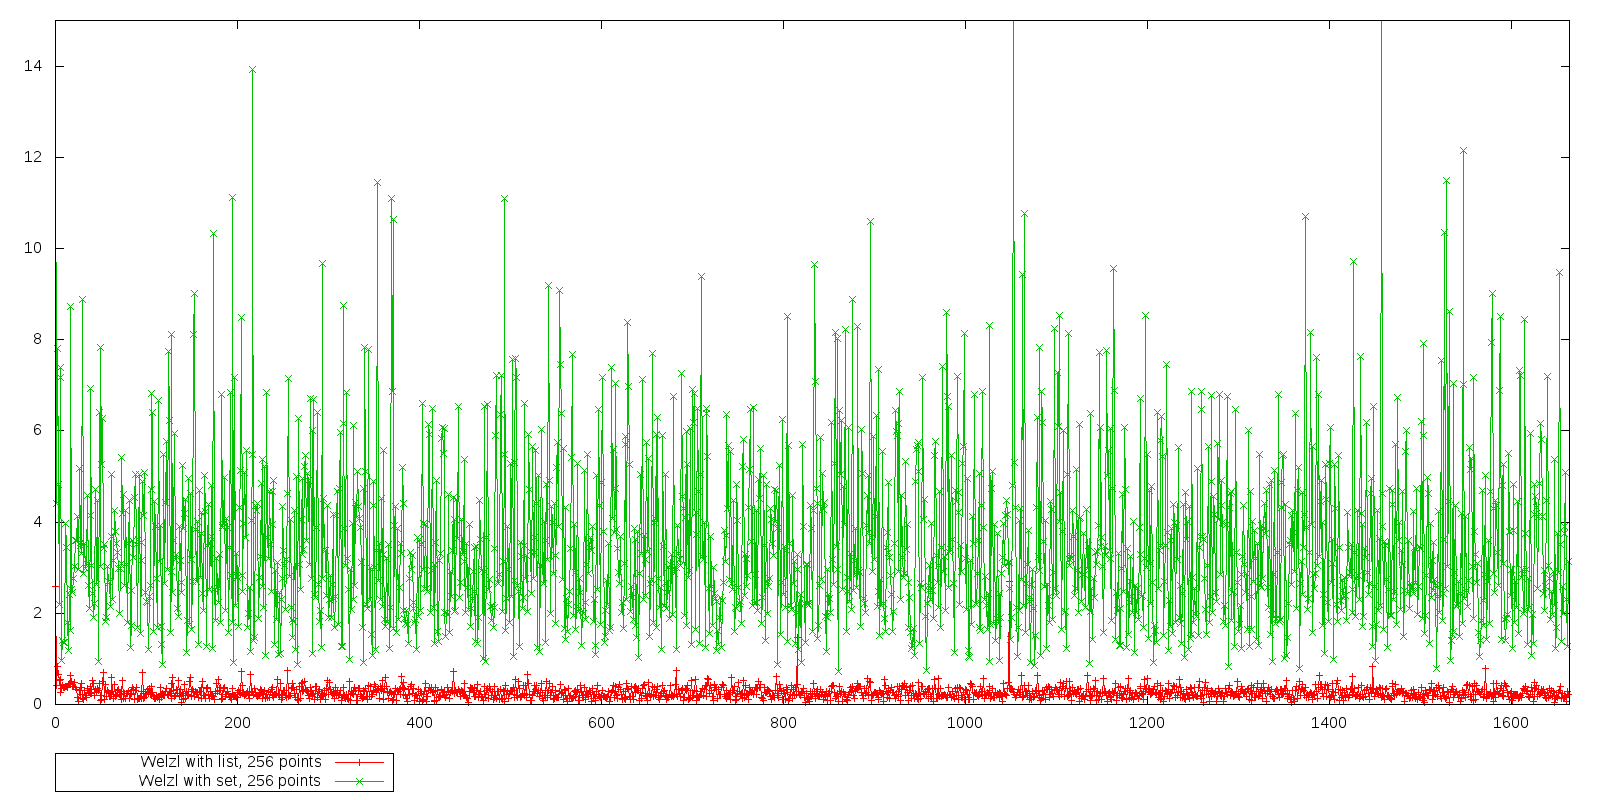
\includegraphics[width=\linewidth]{img/set-vs-list2.png}
Dû au nombre de collisions, et donc à un accès non constant, la HashSet en vert est la moins performante, en plus d'avoir une variance importante.\\
L'ArrayList a quand à elle une variance faible, avec une bonne performance.\\
Nous utiliserons donc des ArrayList pour les résultats suivants.\\
\subsection{En fonction de l'algorithme}
Nombre de points par instance en fonction du temps (millisecondes) :\\
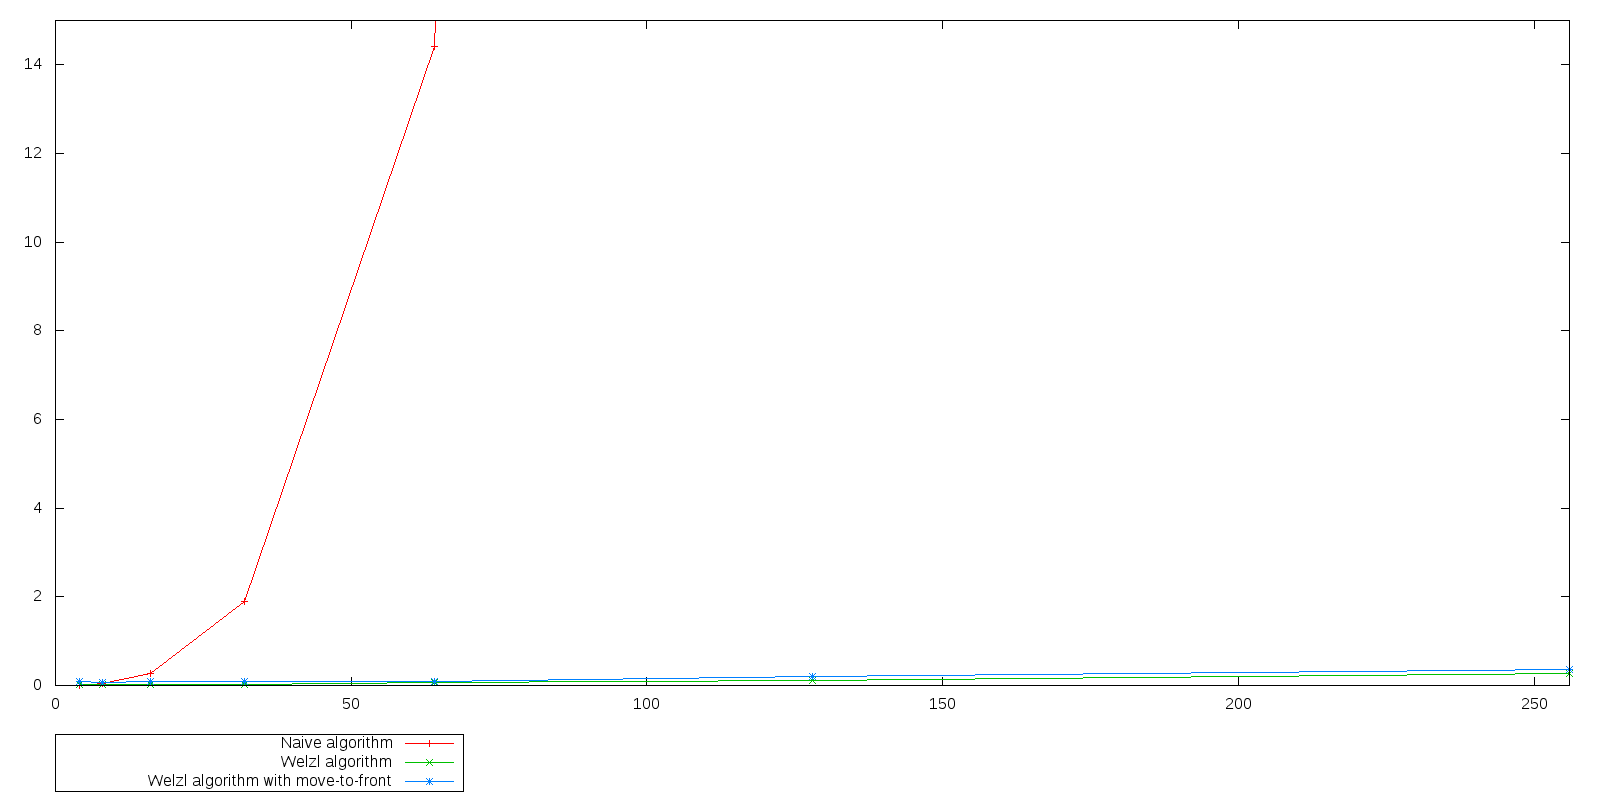
\includegraphics[width=\linewidth]{img/naif-welzl-mtf.png}
Ces calculs sont basés sur la moyenne de 1664 tests pour chacune des instances suivantes : 4,8,16,32,64,128,256.\\
L'algorithme naïf a un très mauvais score, comme attendu.\\
Nos expérimentations rentrent en accord de l'article de Welzl, qui indique un temps expérimental significativement meilleur en utilisant une méthode de "move-to-front". En effet, en sélectionnant un indice aléatoire dans notre ArrayList, nous parvenons à un résultat légèrement meilleur. Il semble en revanche difficile d'analyser pourquoi, la différence vient peut-être des progrès récents dans la génération de nombres aléatoires.\\
L'algorithme de Welzl admet en revanche un temps linéaire comme convenu, malgré son analyse théorique en $\mathcal{O}(N^2)$
\subsection{Comparaison des méthodes de Welzl}
Comparaison des méthodes de choix aléatoire et de "move-to-front" en focntion du temps (millisecondes).\\
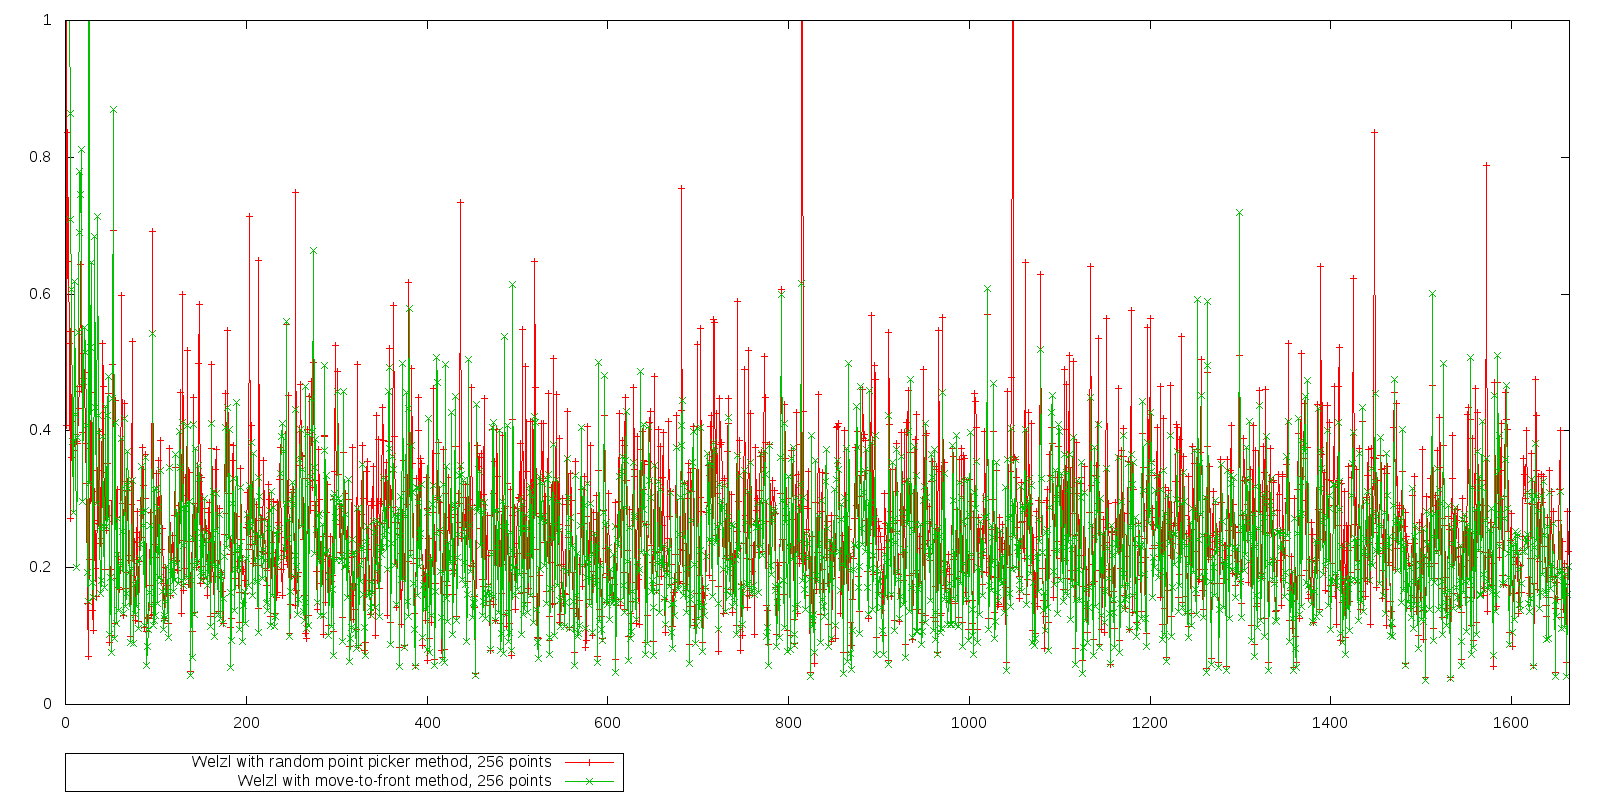
\includegraphics[width=\linewidth]{img/mtf-vs-perm.png}
Les deux méthodes semblent équivalentes au point de vue de la variance.\\
Nous venons de voir précédemment que la méthode du move-to-front semble en revanche légèrement moins performante.\\


\section{Discussion}
\subsection{Peut-on faire mieux ?}
Il semble difficile de faire mieux. Les améliorations possibles doivent certainement se trouver au niveau du choix des points pour la création d'un cercle afin d'éviter des cercles qui ne peuvent contenir la solution. Connaître un ordre de grandeur de la répartition des points avant de lancer l'algorithme pourrait aider, tout en essayant de prendre des points sur l'enveloppe convexe du nuage.\\
Il est peut-être possible de paralléliser un algorithme en séparant un nuage en plusieurs sous ensembles, mais ceci reste à montrer.\\
\subsection{Extension vers $\mathcal{R}^d$}
L'algortihme de Welzl s'appliquera très bien à une sphère, et même vers des dimensions plus grandes. La différence résidera dans la première condition puisque la condition R==3 équivaut en fait à R==(d+1) où d est la dimension considérée. En effet il suffit de trois points pour caractériser un cercle, 4 points pour une sphère, etc... !\\
Concernant la complexité, celle-ci devrait rester dans un temps linéaire. Pour un nombre de points équivalent, nous devrions essayer autant de sphère que nous avons essayé de cercle pour résoudre le problème.\\

\section{Conclusion}
 L'algorithme de Welzl est donc un algorithme performant, en fait le plus performant à ce jour, et qui a le mérite de donner un cercle minimal exact. Il faut toutefois faire attention au choix de la structure de données pour contrôler sa performance au maximum. D'après nos résultats, une implémentation avec une ArrayList (tableau dynamique) avec une méthode de choix du point aléatoire dans l'ensemble.\\
 
 
 \section{Référence}
  [1] Emo Welzl. Smallest enclosing disks (balls and ellipsoids). In H. Maurer, editor, New Results and New Trends in Computer Science, volume 555 of Lecture Notes Comput. Sci., pages 359–370. Springer-Verlag, 1991.\\
\end{document}